\documentclass[12pt,a4paper]{article}

\usepackage[spanish,es-tabla]{babel}
\usepackage[a4paper,bindingoffset=0.1in,%
left=0.75in,right=0.75in,top=1in,bottom=1in,%
footskip=.2in]{geometry}
\usepackage[utf8]{inputenc} % Escribir con acentos, ~n...
\usepackage{eurosym} % s´ımbolo del euro
\newcommand{\horrule}[1]{\rule{\linewidth}{#1}} % Create horizontal rule command with 1 argument of height
\usepackage{listings}             % Incluye el paquete listing
\usepackage[cache=false]{minted}
\usepackage{graphics,graphicx, float} %para incluir imágenes y colocarlas
\usepackage{hyperref}
\hypersetup{
	colorlinks,
	citecolor=black,
	filecolor=black,
	linkcolor=black,
	urlcolor=black
}
\usepackage{multirow}
\usepackage{array}
\usepackage{diagbox}
\usepackage{amsmath}
\usepackage{verbatim}
\begin{document}

\title{Simulación de Sistemas. Ejercicio 2}

\author{
  Antonio Jesús Heredia Castillo\\
}

\date{}
\maketitle
\horrule{2pt}
\section{Modelo diseñado}
Para este ejercicio, me he basado en el sistema creado en practicas de colas en un servidor (colmmk). La diferencia de ese ejemplo y el que estamos usando en este ejercicio es uno básico.  Y es que en aquel ejemplo solo pasaba por un servidor. En este ademas de que pasa por dos servidores, primero por A y luego por B, cada uno tiene distintos tipos de servicio. Como se puede pensar de forma intuitiva, en este ejercicio vamos a necesitar un suceso mas, al que se llega después de pasar por el segundo servidor.
\section{Grafo de sucesos}

Los suceso que tendrá mi sistema son:
\begin{enumerate}
	\item \textbf{suceso\_llegada}: Es por el primer suceso que pasa cuando llega al servidor. Y se esta esperando a ser atendido por el servidor A.
	\item \textbf{suceso\_fin\_a}: Cuando termina en el servidor A y empieza a esperar (o no) a ser servido por B.
	\item \textbf{suceso\_fin\_b}: Termina su paso por el servidor B.
	\item \textbf{suceso\_finsimulacion}: Cuando termina la simulación.
\end{enumerate}
\newpage
El grafo de suceso quedara de la siguiente forma:
\begin{figure}[ph]
	\centering
	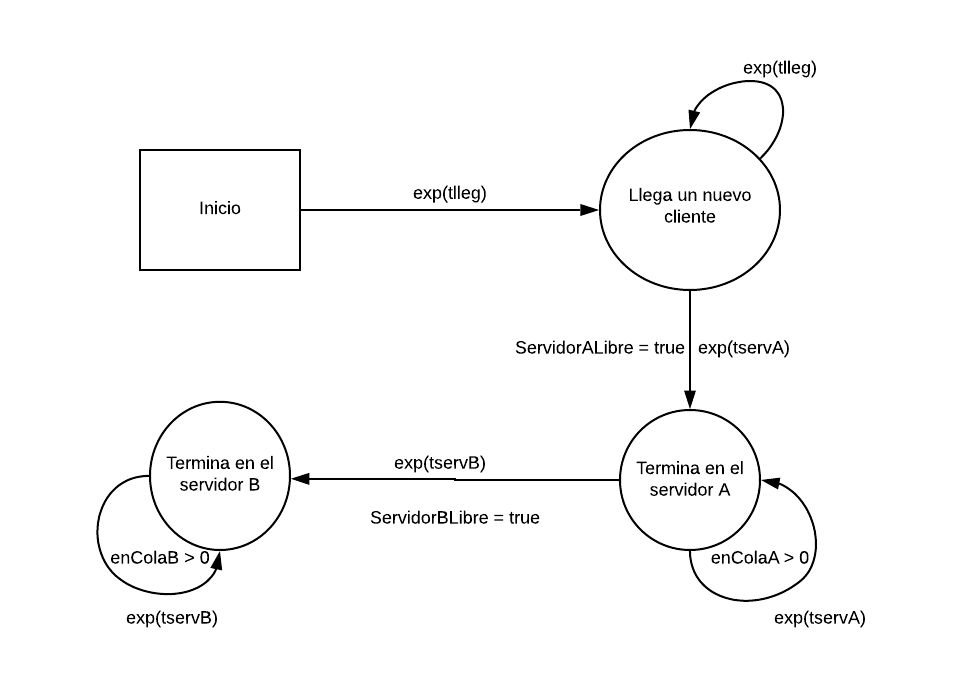
\includegraphics[width=0.7\linewidth]{./BlankDiagram.png}
	\caption{Grafo de sucesos}
	\label{fig:blank-diagram}
\end{figure}
Las constantes tendrán las siguientes valores como se describen en el enunciado del ejercicio.
\begin{itemize}
	\item $tlleg=1.0$
	\item $tservA=0.8$
	\item $tservB=1.2$	
\end{itemize}
\section{Detalle de las rutinas y variables mas destacadas}
Tenemos varias constantes para el uso de nuestro sistema:
\begin{itemize}
\item \textbf{suceso\_llegada}: definición del tipo de suceso de llegada.
\item \textbf{suceso\_fin\_a}: definición del tipo de suceso de fin del uso del servidor A.
\item \textbf{suceso\_fin\_a}: definición del tipo de suceso de fin del uso del servidor B.
\item \textbf{suceso\_finsimulacion}: definición del tipo de suceso de finalización de la simulación.
\end{itemize}
En el programa usamos varias variables para poder llevar el sistema de simulación. A continuación detallo las mas importantes:
\begin{itemize}
	\item \textbf{Actual} suceso actual en la simulación.
	\item \textbf{enColaServA} cantidad de clientes que hay en la cola del servidor A.
	\item \textbf{enColaServB} cantidad de clientes que hay en la cola del servidor B.
	\item \textbf{libreA} si el servidor A esta libre.
	\item \textbf{libreB} si el servidor B esta libre.
	\item \textbf{nClientAntent} el numero total de clientes atendidos.
	\item \textbf{tTotalEnSistema} el tiempo total que han pasado los clientes en el sistema. 
	\item \textbf{lsuc} lista de sucesos.
	\item \textbf{tLlegadas} lista de tiempos de llegadas.
\end{itemize}
Por no añadir código en la memoria, pondré el nombre de las funciones mas importantes que uso en el programa y daré una pequeña explicación de cada una.\\
La función "void suceso()" es la que con un switch-case, decidirá, según el suceso Actual.\\
La función "void iniciar\_variables()"  es donde iniciaremos todas las variables con los siguientes valores: 
\begin{itemize}
	\item \textbf{reloj} = 0.
	\item \textbf{tParada} = 0.
	\item \textbf{enColaServA} = 0.
	\item \textbf{enColaServB} = 0.
	\item \textbf{libreA} = true.
	\item \textbf{libreB} = true.
	\item \textbf{nClientAntent} = 0.
	\item \textbf{tTotalEnSistema} = 0.
	\item \textbf{lsuc}.clear().
	\item \textbf{tLlegadas}.clear().
\end{itemize}
La función "void suceso\_fin()" sera la encargada de finalizar la simulación. Se modifica la variable de finalización y ademas se calcula el tiempo medio de esa ejecución añadiendolo a la lista de tiempos medios.\\
\\
La función "void suc\_fin\_b()" sera la función que se ejecute cuando el suceso finalice en el servidor B. Aquí añadimos uno al numero de clientes que han pasado por el sistema, sumamos el  tiempo que el cliente ha pasado en el sistema. Ademas si queda algún cliente en la cola del servidor B, añadimos un nuevo suceso de salida del servidor B. Si no hay clientes en cola indicamos que el servidor esta libre.\\\\

La función "void suc\_fin\_a()" si hay clientes en la cola del servidor A, se genera un nuevo suceso para que pase el siguiente cliente, si no hay nadie se indica que el servidor esta libre. En caso de que el servidor B este libre se pasa el cliente al servidor B en caso de que no este libre se añade un nuevo cliente a la cola de ese servidor.\\\\

La función "void\ llegaServ()"  es la que se ejecuta conn el suceso de llegada de un nuevo cliente. Lo primero que se hace es añadir el tiempo de llegada de ese cliente al servidor para luego calcular el tiempo de estancia y se añade ese suceso. Si el servidor A ya esta libre, se inserta el suceso de fin del servidor A que equivale a que el cliente ya ha entrado y terminado en ese servidor. Si no esta libre se añade un nuevo cliente a la cola del servidor. \\\\
Ademas tenemos varias funciones para el uso simplificado del programa. Ademas también esta la función de generador exponencial usado en la practica 3 en el código "colmmark". 

La función que uso para mostrar el informe simplemente suma todos los tiempos medios  y calcula la media de todas las simulaciones realizadas. 
\section{Experimentación}
Lo primero que he realizado era ver que resultado nos daba la ejecución del sistema con las condiciones iniciales. Usando una sola simulación como podemos ver en la siguiente tabla, da resultados muy dispares.
\begin{table}[H]
	\centering
\begin{tabular}{|c|c|}
	\hline 
	Nº Ejecución & Tiempo medio de espera \\ 
	\hline 
	1 & 53 \\ 
	\hline 
	2 & 43 \\ 
	\hline 
	3 & 29 \\ 
	\hline 
	4 & 62 \\ 
	\hline 
	5 & 73 \\ 
	\hline 
\end{tabular} 
\end{table}
Como suele pasar en este tipo de problemas realizando un numero de simulaciones mas elevado (en este caso 1000)suele dar unos valores menos dispares como podemos ver en la siguiente tabla.
 \begin{table}[H]
	\centering
\begin{tabular}{|c|c|}
	\hline 
	Nº Ejecución & Tiempo medio de espera \\ 
	\hline 
	1 & 46.32 \\ 
	\hline 
	2 & 46.23 \\ 
	\hline 
	3 & 45.544 \\ 
	\hline 
	4 & 45.961 \\ 
	\hline 
	5 & 46.597 \\ 
	\hline 
\end{tabular} 
\end{table}
Ahora realizaremos varias pruebas para ver como afecta la disminución del \textbf{tservB} hasta que baje de los 10 minutos el tiempo medio de espera. 
 \begin{table}[H]
	\centering
\begin{tabular}{|c|c|}
	\hline 
	tServB & Tiempo medio de espera \\ 
	\hline 
	1.2 & 46.244 \\ 
	\hline 
	1.1 & 31.773 \\ 
	\hline 
	1 & 18.545\\ 
	\hline 
	0.9 & 10.139 \\ 
	\hline 
	0.85 & 8.289 \\ 
	\hline 
\end{tabular}
\end{table}
Como con un valor de \textbf{0.9} aunque es por muy poco, todas las ejecuciones que he realizado estan por encima de 10 minutos, para asegurar que el tiempo medio de espera sea inferior a 10 minutos podemos poner un \textbf{tServ=0.85}. 
\end{document}
